% ==============================================================================
\chapter{Thin sensors studies}
\label{ch:ThinSensorsStudies}
%==============================================================================    

\section{Active-edge sensors}

Thin n-in-p planar sensors produced by
Advacam~\cite{AdvacamRef} are bump bonded to the Timepix3
readout chips ($55\,\micron$ pixel pitch) and studied in test beams
and simulations.  Active-edge sensors allow for seamless tiling of
pixel matrices in large areas of a vertex detector by depleting them
to their physical edge. This allows for high coverage without creating
overlaps between the pixel matrices and therefore reduces the
material. Planar n-in-p pixelated sensors with active edge using a
Deep Reactive Ion Etching (DRIE) process have been produced. This
process consists of extending the backside implantation to the
edge. Figure~\ref{fig:activeedge} illustrates a cross section
of an active-edge sensor with and without guard ring. Since the
back-side voltage is extended to the edge of the sensor, the gradient
of potential between the edge and the last pixel can be very high and
could lead to a breakdown of the sensor. A guard ring consists of an
n-implant with a metallic contact on top of it surrounding the pixel
matrix close to the edge and thereby smoothening the potential
transition between the edge and the neighbouring pixels. The potential
of the guard ring can be floating or grounded by connecting it to the
ground of the readout ASIC. Timepix3 ASICs provide an extra row of
bumped pixels allowing to connect the guard ring to ground.


\begin{figure}[htbp]
  \begin{center}
    \begin{tikzpicture}
      \node[anchor=south west,inner sep=0] (image) at
      (0,0){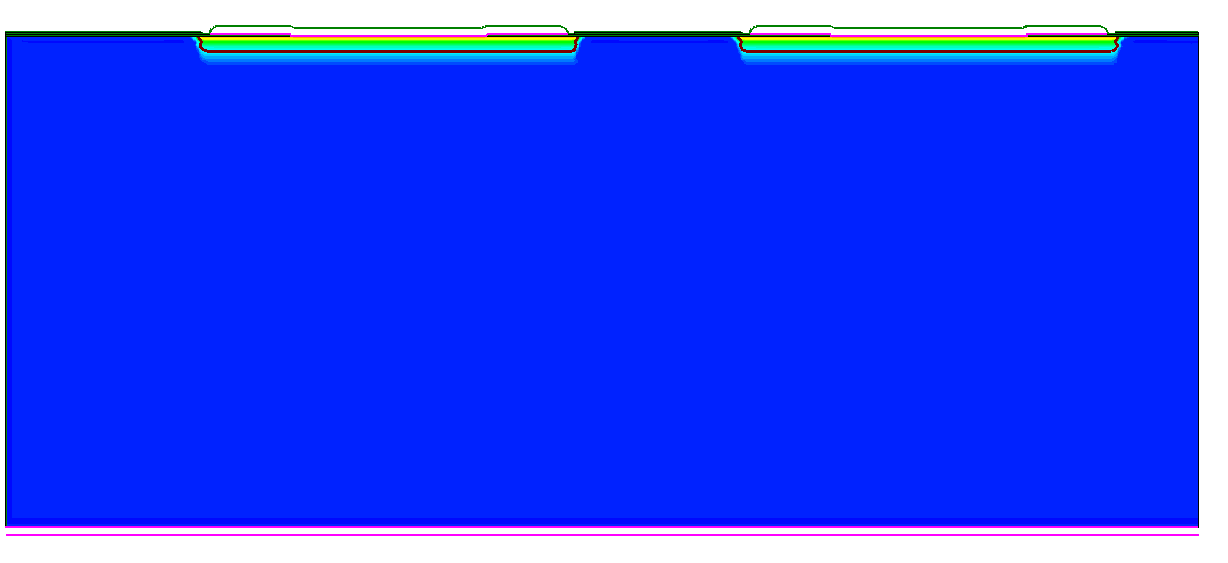
\includegraphics[width=.6\textwidth]{figures/ActiveEdge/schematic.png}};
      \begin{scope}[x={(image.south east)},y={(image.north west)}]
        \draw[-, dashed, line width=.7pt, color=white](0.1, 0.05) -- (0.1, 0.92);
        \draw[-, dashed, line width=.7pt, color=white](0.54, 0.05) -- (0.54, 0.92);
        \draw[<->, line width=.7pt, color=black](0.01, 0.97) -- (0.16, 0.97); % edge width
        
        \node[above, color=black] at (0.05, 0.97) {edge (20 \micron)};
        
        \draw[<->, line width=.4pt, color=black](0.17, 0.97) -- (0.47, 0.97); % n-implant
        \node[above, color=black] at (0.33, 0.97) {n-implant (36 \micron)};
        \node[above, color=white] at (0.3, 0.5) {p-substrate};
        \draw[<->, line width=.4pt, color=black](0.54, 0.0) -- (0.98, 0.0); % pixel width
        \node[below, color=black] at (0.75, 0.0) {pixel (55 \micron)};
        
        \draw[-, line width=3pt, color=violet](0.0, 0.05) -- (0.98, 0.05); % p+ backside contact
        \node[below, color=violet] at (0.15, 0.0) {p+ backside contact};
        \draw[-, line width=3pt, color=violet](0.0, 0.045) -- (0.0, 0.93); % p+ active-edge contact
        \node[left, color=violet, rotate=90] at (-0.05, 0.7) {p+ active edge};
        \node[left, color=white, rotate=90] at (0.08, 0.7) {final pixel edge};

        % \draw[help lines,xstep=.1,ystep=.1] (0, 0) grid (1,1);
        % \foreach \x in {0,1,...,9} { \node [anchor=north] at (\x/10,0) {0.\x}; }
        % \foreach \y in {0,1,...,9} { \node [anchor=east] at (0,\y/10) {0.\y}; }

      \end{scope}
    \end{tikzpicture}
    \caption{Schematic showing the cross section of a sensor with
      $20\,\micron$ active-edge technology. The pixel edges considered
      in the analysis are indicated with dashed lines.}
    \label{fig:activeedge}
  \end{center}
\end{figure}


\begin{table}[htbp]
  \centering
  \caption{Advacam active-edge n-in-p planar pixel sensor assemblies. The edge distance is defined by the distance between the last pixel implant and the physical sensor edge.}
  \label{tab:activeEdgeAssembliesList}
  \begin{tabular}{lccc}
    \toprule
    Assembly & Thickness [\micron] & Edge distance [\micron] & ID \\
    \midrule
    20-NGR  & 50 & 20 & W19\_G7 \\
    23-FGR & 50 & 23 & W19\_F7 \\ \hline
    28-GNDGR & 50 & 28 & W19\_L8 \\
    55-GNDGR & 50 & 55 &W19\_C7 \\
    55-GNDGR-100 & 100 & 55 & W5\_E2  \\ \hline
    55-GNDGR-150 & 150 & 55 & W5\_F1 \\
    \bottomrule
  \end{tabular}
\end{table}

The IV measurement is shown in Figure~\ref{fig:IVmeasurements}.

\begin{figure}[htbp]
  \centering
  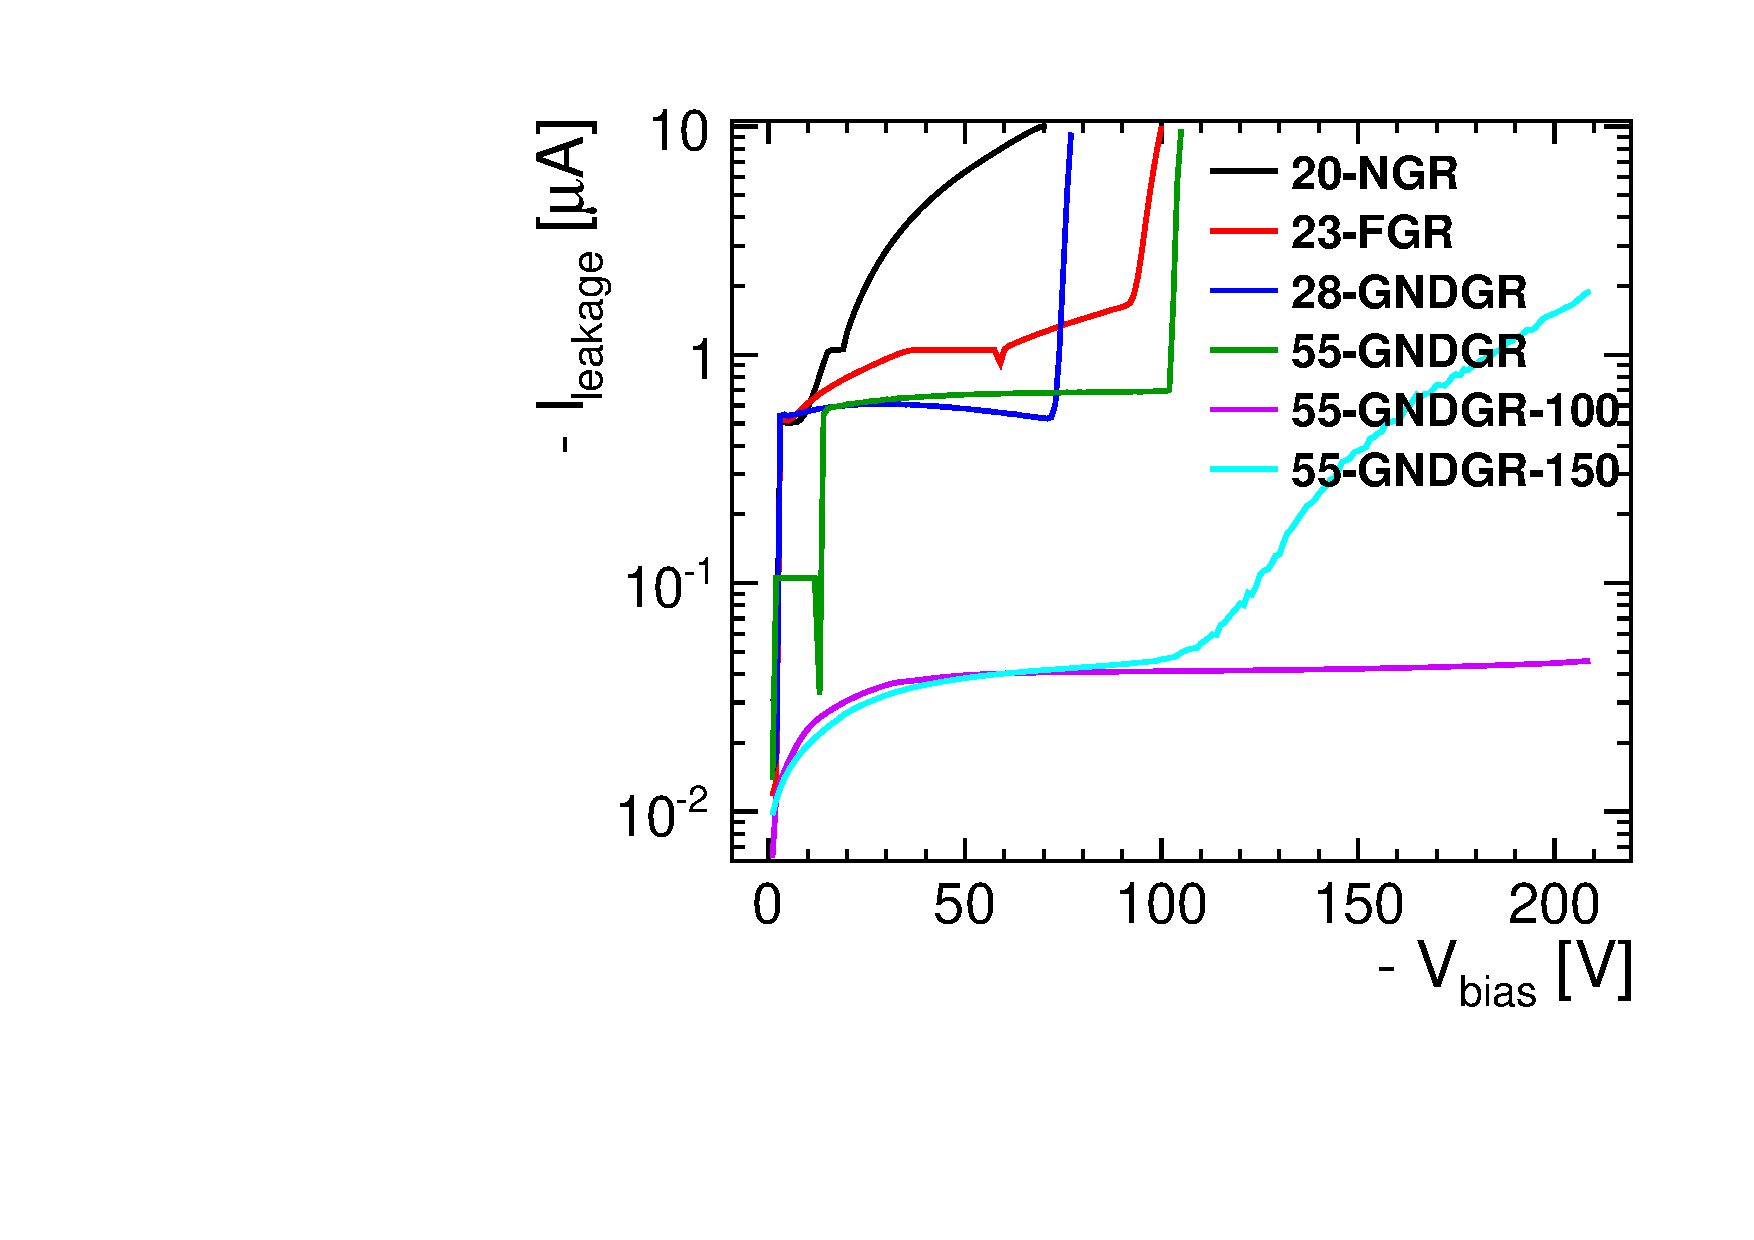
\includegraphics[width=0.7\textwidth]{figures/ActiveEdge/IVCurve.pdf}
  \caption{IV measurements for the assemblies listed in Table~\ref{tab:activeEdgeAssembliesList}.}
  \label{fig:IVmeasurements}
\end{figure}

The layers in the geometry description are defined in
Figure~\ref{fig:PixelLayout} and explained in
Table~\ref{tab:PixelStackDimensions}.

\begin{figure}[htbp]
  \centering
  \begin{minipage}[t]{.4\textwidth}
    \centering
    \vspace{0pt}
    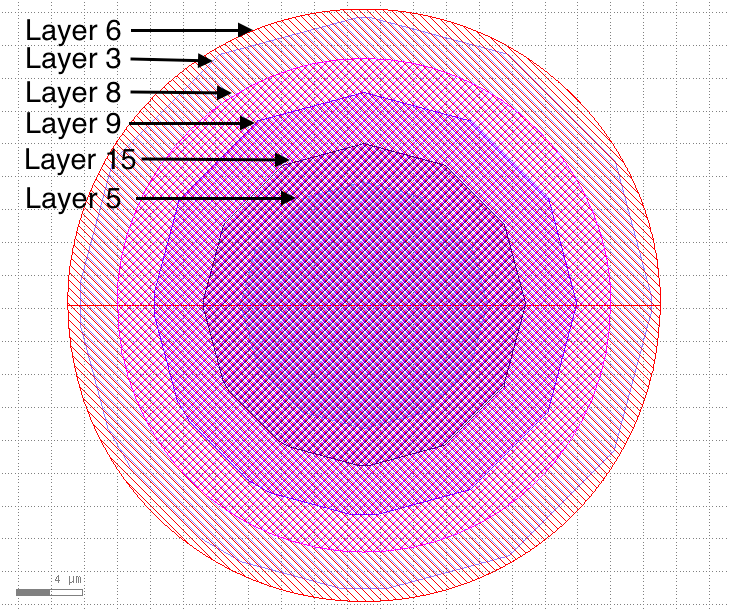
\includegraphics[width=0.95\textwidth]{figures/ActiveEdge/pixelLayout_withLayers.png}
    \caption{}
    \label{fig:PixelLayout}
  \end{minipage}
  \hfill
  \begin{minipage}[t]{.56\textwidth}
    \centering
    \vspace{0pt}
    \captionof{table}{Layers in the sensor from the gds file
      (Picture from 23-FGR).}
    \label{tab:PixelStackDimensions}
    \begin{tabular}{l c c}
      \toprule
      Layer number & Layer \\
      \midrule
      6 & metal\\
      3 & - \\
      8 & implant \\
      9 & UBM (for thin film lift off metal) (??) \\
      15 & passivation \\
      5 & contact to connect Al to Si \\
      \bottomrule
    \end{tabular}
  \end{minipage}
\end{figure}

Table~\ref{tab:DimensionsForAssemblies} summarises the dimensions of
the implants for the sensors. The edge width is the distance between
the last pixel implant to the physical edge of the sensor. The metal
width is the diameter of the metal for the pixels. The doping width is
the diameter of the pixels implant. The contact width is the diameter
of the contact between silicon and the metal (where the oxide is
etched). The GR offset is the distance between the physical edge of
the sensor and the implant of the GR.

\begin{table}
  \centering
  \captionof{table}{The pixels and guard-ring dimensions for different assemblies}
  \label{tab:DimensionsForAssemblies}
  \begin{tabular}{l c c c c}
    \toprule
    & 20-NGR & 23-FGR & 28-GNDGR & 55-GNDGR \\
    \midrule
    Edge width [\micron] & 20 & 23 & 28 & 55 \\
    Metal width [\micron] & 40 & 36 & 36 & 40 \\
    Doping width [\micron] & 30 & 30 & 30 & 30 \\
    Contact width [\micron] & 15 & 15 & 15 & 15 \\
    GR offset [\micron] & - & 10 & 14.5 & 25 \\
    GR doping width [\micron] & - & 5 & 5 & 5 \\
    GR contact width [\micron] & - & 3 & 3 & 15 \\
    GR metal width [\micron] & - & 7 & 7 & 10 \\
    \bottomrule
  \end{tabular}
\end{table}






For the 50~\micron grounded GR, the dimensions of the pixels are
differente from above.
\captionof{table}{Layers and dimensions from the gds geometry
  (taken from Timepix 20um GR FLOAt and from Timepix 50~\micron grounded GR).}
\label{tab:PixelStackDimensions}
\begin{tabular}{l c c c}
  \toprule
  Layer number & Layer & Diameter (20 float) [\micron] & Diameter (50 GND) [\micron]\\
  \midrule
  6 & metal & 36 & 40 \\
  3 & - & 34.62 & 36 \\
  8 & implant & 30 & 30 \\
  9 & UBM & 25.6 & 25.6 \\
  15 & passivation & 19.5 & 19.5 \\
  5 & contact to connect Al to Si & 15 & 15 \\
  \bottomrule
\end{tabular}




\begin{figure}[htbp]
  \centering
  \begin{subfigure}[b]{0.33\textwidth}
    \centering
    \fbox{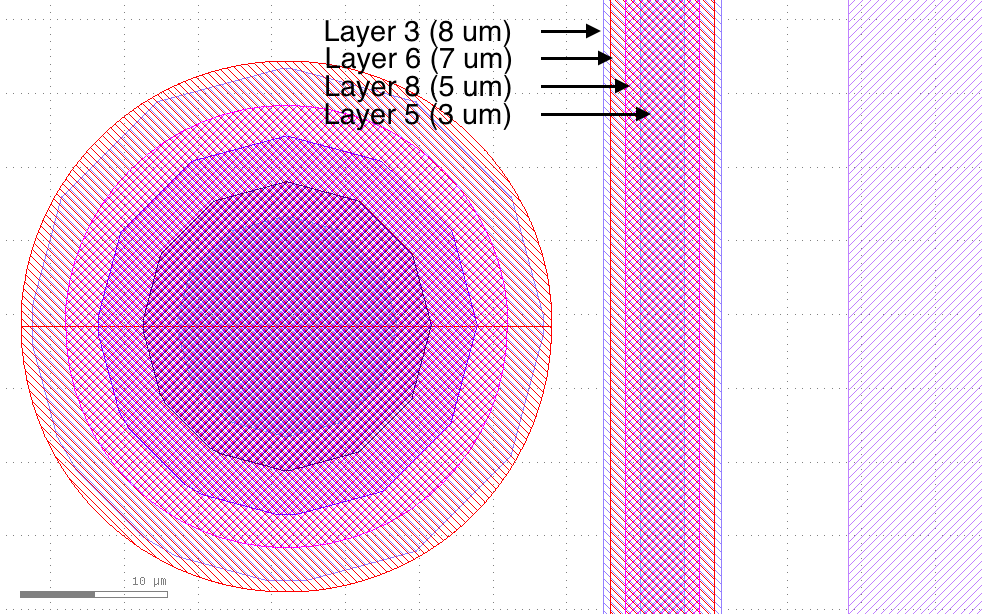
\includegraphics[width=0.95\textwidth]{figures/ActiveEdge/20umEdge_float_GR_withText.png}}
    \caption{20~\micron edge: Floating guard ring}
    \label{fig:GuardRingLayout_20_float_GR}
  \end{subfigure}\hfill
  \centering
  \begin{subfigure}[b]{0.33\textwidth}
    \centering
      \fbox{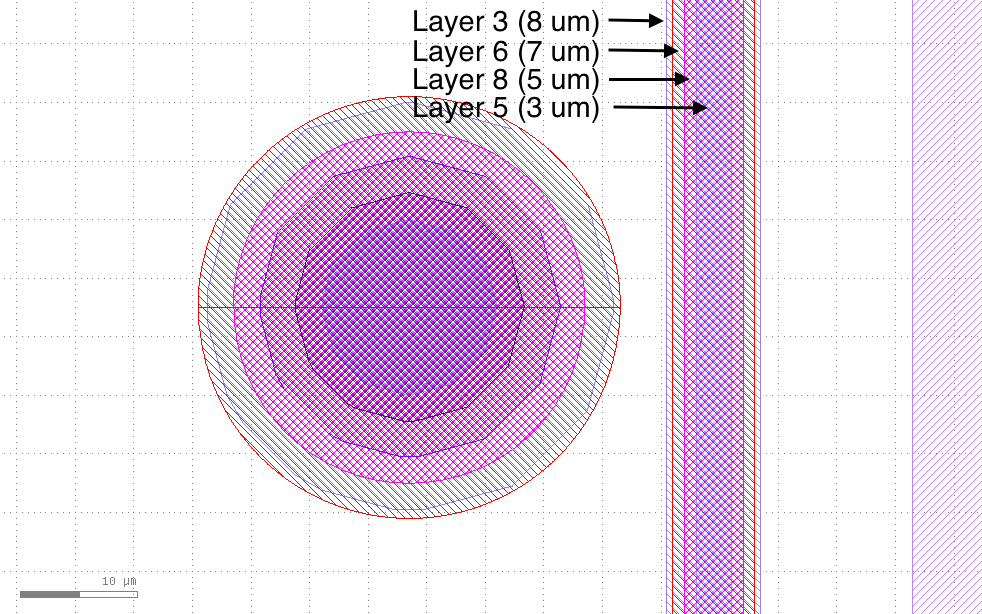
\includegraphics[width=0.95\textwidth]{figures/ActiveEdge/20umEdge_GND_GR_withText.png}}
    \caption{20~\micron edge: GND guard ring}
    \label{fig:GuardRingLayout_20_GND_GR}
  \end{subfigure}\hfill
  \centering
  \begin{subfigure}[b]{0.33\textwidth}
    \centering
    \fbox{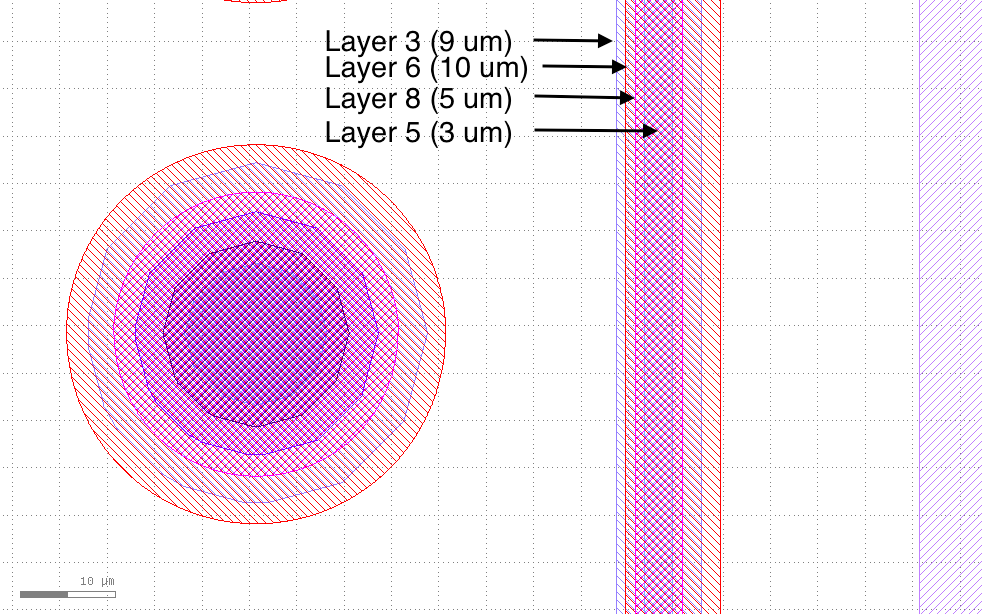
\includegraphics[width=0.95\textwidth]{figures/ActiveEdge/50umEdge_GND_GR_withText.png}}
    \caption{50~\micron edge: GND guard ring}
    \label{fig:GuardRingLayout_50_GND_GR}
  \end{subfigure}
  \label{fig:GuardRingLayout}
\end{figure}


% \begin{figure}[htbp]
%   \centering
%   \begin{minipage}[t]{.4\textwidth}
%     \centering
%     \vspace{0pt}
%     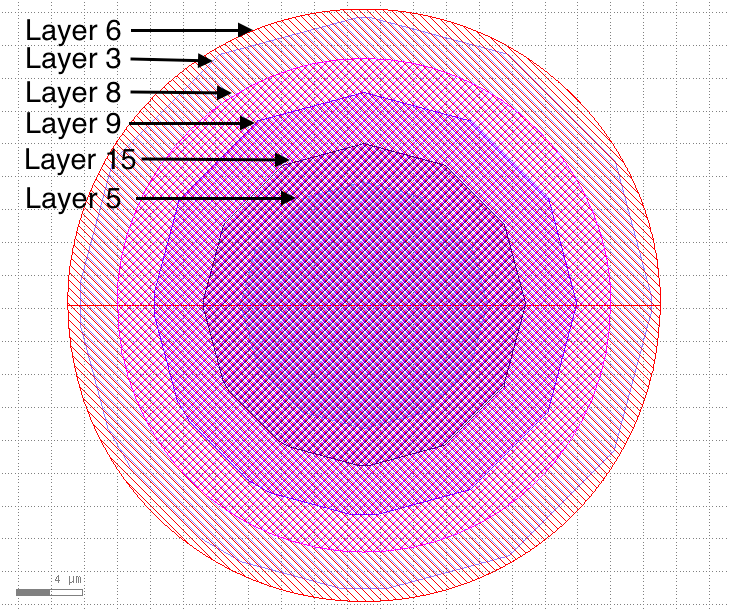
\includegraphics[width=0.95\textwidth]{figures/ActiveEdge/pixelLayout_withLayers.png}
%     \caption{}
%     \label{fig:PixelLayout}
%   \end{minipage}
%   \hfill
%   \begin{minipage}[t]{.56\textwidth}
%     \centering
%     \vspace{0pt}
%     \captionof{table}{Layers and dimensions from the gds geometry
%       (taken from Timepix 20um GR FLOAT).}
%     \label{tab:PixelStackDimensions}
%     \begin{tabular}{l c c}
%       \toprule
%       Layer number & Layer & Diameter [\micron]\\
%       \midrule
%       6 & metal & 36 \\
%       3 & - & 34.62 \\
%       8 & implant & 30 \\
%       9 & UBM (for thin film lift off metal) (??) & 25.6 \\
%       15 & passivation & 19.5 \\
%       5 & contact to connect Al to Si & 15 \\
%       \bottomrule
%     \end{tabular}
%   \end{minipage}
% \end{figure}